\chapter{Fundamentação Teórica}\label{cap_fundamentos}

Este capítulo abrange conceitos relacionados ao entendimento do trabalho e que contextualizam um \textit{Business Intelligence} com suas principais características e aplicações, como também em posterior os principais conceitos e funções da nutrição no ambiente hospitalar. 

% ---
\section{\textit{Business Intelligence}}
% ---
O \textit{Business Intelligence} (BI) é um conjunto de conceitos e metodologias que apoiam a tomada de decisão a partir de dados obtidos na organização. Um guarda-chuva conceitual, segundo \citeonline{barbieri2011}, pois visa coletar dados, informações e conhecimentos que permitem às empresas competirem de forma mais eficaz em uma abordagem evolutiva da modelagem de dados, capaz de promover a estruturação da informação em depósitos retrospectivos e históricos, permitindo que sejam modelados com ferramentas analíticas. Seu conceito é abrangente e inclui todos os recursos necessários para processar e compartilhar informações com o usuário.

Um ponto importante a ser salientado, é de que um projeto de BI pode proporcionar ganhos não somente aos gestores das organizações, mas também a determinados departamentos que precisem se basear em informações concretas para tomar decisões satisfatórias \cite{antonelli2009}.

É preciso ter em mente que um sistema de BI não existe por si só, ele está estreitamente ligado às fontes de dados subjacentes, sejam sistemas transacionais ou planilhas de suporte, em suma, tudo o que pode ser considerado um repositório primário de dados resultantes de processos de negócio da organização \cite{sezoes2006}. De forma técnica o conjunto integrado de ferramentas, tecnologias e produtos de software que são usados para coletar dados, integrá-los e analisá-los, inclui, segundo \citeonline{olszakziemba2012}:

\begin{itemize}
     \item ferramentas para extrair, transformar e carregar dados (ferramentas ETL, \textit{Extration - Transformation - Load}) - são as principais responsáveis pela transferência de dados de sistemas de transação, planilhas e arquivos para \textit{Data Warehouses};
     \item \textit{Data Warehouses} - proporcionam local para armazenamento temático de dados agregados e já analisados;
     \item ferramentas analíticas (\textit{On-line Analytical Processing}) - permitem que os usuários acessem, analisem e modelem problemas de negócios e compartilhem informações armazenadas em \textit{Data Warehouses};
     \item ferramentas de mineração de dados - permitem descobrir vários padrões, generalizações, regularidades e regras em recursos de dados;
     \item ferramentas para relatórios e consultas \textit{ad hoc} - permitem a criação e utilização de diferentes relatórios sintéticos;
     \item camada de apresentação - aplicações que incluem interfaces gráficas e multimídia cuja tarefa é fornecer informações aos usuários de forma confortável e acessível.
\end{itemize}

Os itens anteriormente citados, serão melhor detalhados nas subseções \autoref{subD-etl}, \autoref{subD-datawarehouse}, \autoref{subD-olap}, \autoref{subD-relatorios} e \autoref{subD-relatorios}.

% ---
\subsection{\textit{Extract, Transform, Load}} \label{subD-etl}
% ---

Para que os dados sejam guiados da fonte para a plataforma BI, existe um processo de carregamento denominado: \textit{extract, transform e load} (ETL). \citeonline{braghittoni2017} define os três estágios do ETL da seguinte forma:
\begin{itemize}
    \item \textbf{\textit{Extract}}: é o processo de extrair dados das fontes de origem de forma periódica, lendo uma ou mais fontes de informação. Além disso, à medida que o processo de carregamento se repete, é necessário lidar com tratamento de erros e avaliar possíveis indisponibilidades;
    \item \textbf{\textit{Transform}}: é o processo pelo qual os dados são processados, colocados em um formato específico, verificados mediante as regras de negócio, calculados e etc., ficando disponíveis para o processo de \textit{load};
    \item \textbf{\textit{Load}}: é o processo de incorporação de dados na plataforma de BI. A inclusão desses dados deve ser feita de modo incremental, uma vez que, com as informações inseridas os dados não podem ser alterados. Entretanto existem técnicas para lidar com essas situações dentro do \textit{Business Intelligence}.
\end{itemize}
% ---
\subsection{\textit{Data Warehouse}} \label{subD-datawarehouse}
% ---
O \textit{Data Warehouse} (DW) é o coração da plataforma de BI. Elé é um banco de dados relacional, contudo é desenhado para responder às pesquisas da forma mais performática possível, sendo chamado também de banco de dados dimensional, em decorrência do desenho ser baseado em dimensões. Diferentemente dos bancos de dados transacionais, onde as formas normais guiam a modelagem de dados, o DW é um banco de dados desnormalizado \cite{braghittoni2017}.

É ainda segundo \citeonline{turban2008}, também, um repositório de dados atuais e históricos de possível interesse aos gestores da organização. Uma coleção de dados orientada por assunto, integrada, variável no tempo e não-volátil, que proporciona suporte ao processo decisório.
% ---
\subsection{\textit{Online Analytical Processing}} \label{subD-olap}
% ---
\textit{Online Analytical Processing} (OLAP) é o termo em inglês para Processamento Analítico Online, o qual refere-se às várias atividades normalmente realizadas por usuários finais em sistemas online. Não há consenso sobre quais atividades são consideradas OLAP, mas normalmente, inclui atividades como gerar e responder a consultas, solicitar relatórios e gráficos \textit{ad hoc} como também fazem parte da sua execução, realizar análises estatísticas e criar apresentações visuais. Muitas pessoas também pensam em análises e apresentações multidimensionais e mineração de dados como atividades OLAP. Basicamente, os produtos OLAP oferecem a capacidade de modelar, analisar e visualizar grandes conjuntos de dados, tanto para sistemas de gerenciamento de banco de dados (SGBD) e, mais comumente, para sistemas de \textit{Data Warehouse}, além de também oferecer uma visão conceitual multidimensional dos dados \cite{turban2008}.

As ferramentas OLAP podem ser implementadas de diversas formas, segundo \citeonline{carvalho2003}, são classificadas em três tipos:
\begin{itemize}
    \item \textit{Multidimensional On-Line Analytical Processing} (MOLAP): na arquitetura MOLAP, os dados são armazenados em um banco de dados multidimensional onde o servidor MOLAP atua e o usuário trabalha, coleta e processa vários dados no servidor. Os dados são armazenados em estruturas de dados de \textit{array} para melhor desempenho ao acessá-los, tornando o armazenamento menor em relação ao espaço usado para armazenar os mesmos dados em um banco de dados relacional. Além de ser uma arquitetura rápida, outra vantagem é o rico e complexo conjunto de funções analíticas presentes em bancos multidimensionais.
    \item \textit{Relational On-Line Analytical Processing} (ROLAP): a arquitetura ROLAP é uma simulação da tecnologia OLAP feita em bancos de dados relacionais, que utilizando uma estrutura relacional tem a vantagem de não limitar o tamanho do armazenamento de dados. Esta ferramenta não usa cubos pré-calculados como a MOLAP. Quando um usuário cria uma consulta na interface gráfica, a ferramenta acessa os metadados ou outros recursos de que dispõe para gerar uma consulta em \textit{Structured Query Language} (SQL) e devolver uma resposta;
    \item \textit{Hybrid On-Line Analytical Processing} (HOLAP): chamada de computação híbrida, consegue combinar a capacidade e escalabilidade das ferramentas ROLAP com o excelente desempenho dos bancos de dados multidimensionais. Por exemplo, supondo uma base de clientes que esteja espalhada por 500 cidades, 23 estados, 5 regiões e um total geral. No nível da cidade, o armazenamento multidimensional resolveria consultas para vendas totais. Se, entretanto, fosse necessário consultar as vendas totais de um determinado cliente, o banco de dados relacional responderia muito mais rápido à solicitação. Esta situação é típica da indicação da arquitetura HOLAP.
\end{itemize}

Segundo \citeonline{turban2008}, para apresentar dados no formato multidimensional, três fatores são levados em consideração: as dimensões, as medidas e o tempo. Para representar esses dados com alguma medida de interesse, são usados cubos de dados. O termo "cubo" se refere ao conjunto de dados altamente correlacionado que é organizado para permitir que os usuários combinem qualquer atributo a fim de criar diferentes visões bidimensionais, um exemplo de cubo é mostrado na \autoref{fig_cuboturban}. Apesar de receber a nomenclatura de cubo, os dados podem ser bidimensionais, tridimensionais ou com apenas uma dimensão.

\begin{figure}[htb]
	\caption{\label{fig_cuboturban}Visão e Análise de cubo.}
	\begin{center}
	    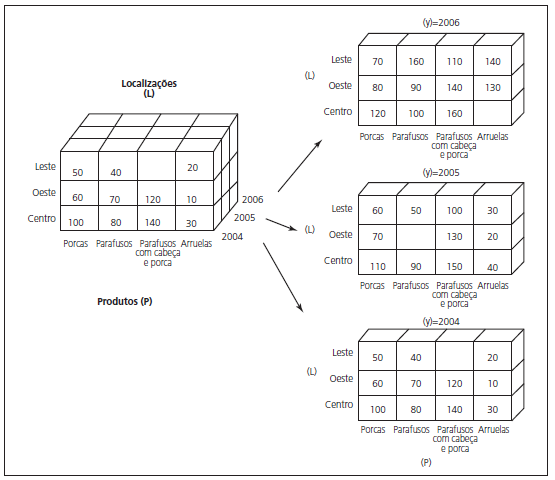
\includegraphics[scale=0.9]{Imagens/figura - cubo olap turban.png}
	\end{center}
	\legend{Fonte: \cite{turban2008}.}
\end{figure}
% ---
\subsection{Ferramentas de apresentação} \label{subD-relatorios}
% ---
As tecnologias visuais podem condensar 1.000 números em uma única imagem e tornar os aplicativos de suporte à decisão mais atraentes e compreensíveis para os usuários. A visualização de dados refere-se a tecnologias que suportam a visualização e às vezes a interpretação de dados e informações em diferentes pontos da cadeia de processamento de dados. Inclui imagens digitais, sistemas geográficos, interfaces gráficas de usuário, gráficos, realidade virtual, representações dimensionais, filmes e animações. Ferramentas visuais podem ajudar a identificar relacionamentos, como tendências \cite{turban2008}.
% ---
\section{\textit{Pentaho Data Integration and Analytics Platform}}
% ---
Os produtos Pentaho fazem parte de uma plataforma abrangente usada para acessar, integrar, manipular, visualizar e analisar dados. Incluem componentes baseados na \textit{web} e ferramentas de \textit{design}. É um projeto de código aberto, desenvolvido em Java e mantido pela Hitachi Vantara© com uma comunidade ativa. A plataforma é oferecida em duas diferentes edições: a \textit{Community Edition}\footnote{\textit{Pentaho Community Edition}: \url{https://sourceforge.net/projects/pentaho/}} e a \textit{Enterprise Edition}\footnote{\textit{Pentaho Enterprise Edition}: \url{https://www.hitachivantara.com/en-us/products/data-management-analytics/pentaho/download-pentaho.html}}. A versão \textit{Community Edition} é distribuída gratuitamente com o foco de ser continuamente desenvolvida de forma cooperativa. A versão \textit{Enterprise Edition} conta com recursos mais avançados como, por exemplo, suporte a dados de \textit{streaming}, biblioteca de conectores ampliada, suporte técnico da Hitachi Vantara, além de outras vantagens prevista no pacote comercial. 

Nesta seção, serão apresentadas as ferramentas disponíveis na versão \textit{Pentaho Community Edition}, necessárias para o desenvolvimento de um projeto de BI.

\subsection{\textit{Pentaho Data Integration}}
\textit{Pentaho Data Integration} (PDI) fornece acesso a um motor de extração, transformação e carregamento (ETL) que captura os dados certos, limpa os dados e armazena os dados usando um formato uniforme que é acessível e relevante para os usuários finais e tecnologias \textit{Internet of Things} (IoT). O cliente PDI é um aplicativo de \textit{desktop} que permite criar transformações e agendar e executar trabalhos \cite{pentahodocumentation}.

Os usos comuns do cliente PDI incluem:
\begin{itemize}
    \item Migração de dados entre diferentes bancos de dados e aplicativos;
    \item Carregar enormes conjuntos de dados em bancos de dados, aproveitando ao máximo os ambientes de processamento em nuvem, em \textit{cluster} e massivamente paralelos;
    \item Limpeza de dados com etapas que variam de transformações muito simples a muito complexas;
    \item Integração de dados, incluindo a capacidade de aproveitar ETL em tempo real como uma fonte de dados para o \textit{Pentaho Reporting};
    \item População do \textit{Data Warehouse} com suporte integrado para alterar lentamente as dimensões e criação de chaves substitutas.
\end{itemize}

\subsection{\textit{Pentaho Schema Workbench}}
\textit{Pentaho Schema Workbench} (PSW) é o software usado para criar esquemas que mapeiam o modelo físico de dados multidimensionais com o modelo lógico do cubo de dados, utilizando o motor OLAP escrito em Java, Mondrian, também desenvolvido pela Pentaho. O PSW constrói a interface entre os modelos a partir de arquivos XML, que são executados pelo Mondrian para realizar as consultas escritas em linguagem \textit{Multidimensional Express} (MDX).

O PSW fornece as seguintes funcionalidades:

\begin{itemize}
    \item Editor de esquema integrado para construção de cubos OLAP;
    \item Teste de consultas MDX nos esquemas e bases de dados.
\end{itemize}

\subsection{\textit{Pentaho Aggregation Designer}}
\textit{Pentaho Aggregation Designer} (PAD) simplifica a criação e implantação de tabelas agregadas que melhoram o desempenho das análises no Pentaho. É uma ferramenta gráfica, desenvolvida em Java, fornece uma interface que permite criar tabelas agregadas de dimensões com níveis, de acordo com a especificação necessária.

\subsection{\textit{Pentaho Business Analytics Platform}}
O \textit{Pentaho Business Analytics Platform} é um ambiente para interação com os dados e administração de usuários da plataforma, também conhecida como \textit{Pentaho Server}. O nome oficialmente empregado pela Hitachi Vantara foi \textit{Pentaho User Console} (PUC). Ele é um ambiente de design baseado na web onde se pode analisar dados, criar relatórios interativos, relatórios de painel e construir painéis integrados para compartilhar soluções de inteligência de negócios com outras pessoas da organização e na internet. Além de seus recursos de design, o \textit{Pentaho User Console} oferece uma ampla variedade de recursos de administração do sistema para configurar o servidor Pentaho, além de administração de permissões de segurança e acesso de usuários.

\subsection{\textit{Pentaho Report Designer}}
\textit{Pentaho Report Designer} (PRD) é uma ferramenta sofisticada para geração de relatórios que pode ser usada independentemente da Suite Pentaho ou integrada ao \textit{Pentaho User Console}. Permite se conectar a múltiplas fontes de dados como, por exemplo, SQL, MDX e \textit{Community Data Access}.

\subsection{\textit{Saiku Analytics}}
\textit{Saiku Business Analytics} é um cliente web OLAP disponível como \textit{plug-in} para o \textit{Pentaho Business Analytics Platform}. Ele utiliza a \textit{engine} Mondrian para explorar as diversas fontes de dados conectadas e proporcionar de forma fácil e amigável o recurso de cubos OLAP com uma experiência simples para usuário final usando tecnologia arrastar e soltar (\textit{Drag and Drop}). 

O \textit{Saiku Analytics} é distribuído pela Meteorite BI© em duas versões, o \textit{Saiku Community Edition}\footnote{\textit{Saiku Community Edition}: \url{https://community.meteorite.bi/}} que é fornecido gratuitamente e a versão \textit{Saiku Enterprise Edition}\footnote{\textit{Saiku Enterprise Edition}: \url{https://www.meteorite.bi/products/saiku/}} que possui suporte comercial.

\section{Terapia Nutricional}
A terapia nutricional (TN) é a intervenção nutricional realizada em pacientes hospitalizados, seguindo um protocolo de rotinas e critérios, e tem como principais objetivos prevenir e tratar a desnutrição, preparando o paciente para o procedimento cirúrgico e clínico, melhorando a resposta imunológica e cicatrizante, modulando a resposta orgânica ao tratamento clínico e cirúrgico, prevenindo e tratando as complicações infecciosas e não infecciosas, como também melhorar a qualidade de vida do paciente, diminuir o tempo de internação, diminuir a mortalidade e, consequentemente, diminuir os custos hospitalares \cite{manualnutricao2016, mcclave2013}. 

Segundo o \citeonline{manualnutricao2016}, existe também um conjunto de ações para a execução da terapia nutricional no paciente, entre elas estão, realizar triagem nutricional, executar avaliação nutricional, calcular necessidades de nutrientes e executar um acompanhamento nutricional até o desfecho da alta médica. O processo mais coerente e produtivo para início da avaliação do estado nutricional em unidades hospitalares é realizar a triagem nutricional \cite{protocolonutricionaladulto}. Na \autoref{subD-triagem} são melhor detalhadas as características da triagem nutricional e algumas atividades subsequentes relevantes para entendimento dos próximos capítulos, são elas, a avaliação nutricional na \autoref{subD-avaliacao} e os indicadores de qualidade em terapia nutricional na \autoref{subD-indicadores}. 

\subsection{Triagem Nutricional} \label{subD-triagem}
Triagem nutricional é definida como um processo de identificação das características conhecidas por estarem relacionadas a problemas nutricionais, com o objetivo de identificar indivíduos desnutridos ou em risco, para que sejam instituídas medidas de intervenção nutricional mais precocemente. Um dos instrumentos de triagem utilizados é o \textit{Nutritional Risk Screening} (NRS). Este instrumento foi desenhado para aplicação em ambiente hospitalar e baseia o rastreamento de risco nutricional nos critérios: perda de peso dos últimos três meses, índice de massa corporal (IMC), ingestão alimentar (apetite e capacidade de se alimentar) e fator de estresse. Um fator de risco adicional para ajustar a classificação de risco é a idade acima de 70 anos \cite{protocolonutricionaladulto, manualnutricao2016}. Para crianças o instrumento indicado pela \textit{European Society of Parenteral and Enteral Nutrition} (ESPEN) é o \textit{Screening Tool for Risk on Nutritional Status and Growth}, cujo termo técnico adotado é \textit{STRONG Kids} \cite{protocolonutricionalinfantil}. 

\subsection{Avaliação Nutricional} \label{subD-avaliacao}
Avaliação nutricional é o exame detalhado das variáveis metabólicas, nutricionais ou funcionais do indivíduo e é realizada quando identificado na triagem algum indicador de risco. É um processo mais longo do que a triagem, onde todas as informações devem ser registradas, datadas e assinadas no prontuário do paciente sendo esta uma atividade de responsabilidade do profissional nutricionista \cite{protocolonutricionaladulto}. 

Assim como para a triagem, existem instrumentos para identificação do estado nutricional de pacientes hospitalizados, segundo \citeonline{baker1982} a Avaliação Subjetiva Global (ASG) e a Avaliação Subjetiva Global Produzida pelo Paciente (ASG-PPP) são exemplos que podem ser aplicados. ASG é um método clínico de avaliação do estado nutricional simples, de baixo custo e não invasivo, aplicado no formato de questionário, que pode ser realizado à beira do leito. Tem fácil execução, boa repetibilidade e é capaz de identificar adequadamente pacientes de maior risco para complicações pós-operatórias ou quando em situações clínicas identifica desnutrição ou risco de desnutrição \cite{baker1982}. Já ASG-PPP é uma forma modificada da ASG, desenvolvida a partir da necessidade de uma aplicação fácil e de baixo custo, porém que pudesse ser utilizada em pacientes oncológicos ambulatoriais \cite{ottery1996}.

\subsection{Indicadores de Qualidade em Terapia Nutricional} \label{subD-indicadores}
O objetivo dos indicadores de qualidade em terapia nutricional é de conhecer a frequência da triagem nutricional desde o primeiro dia de internação, até 48 horas. A meta é atingir pelo menos 80\% do seu resultado. Esse valor pode ser alcançado de forma progressiva, de acordo com a história do estabelecimento hospitalar. Outros indicadores dever ser usados levando em consideração características e necessidades dos indivíduos, sendo relacionados a atributos de simplicidade, objetividade e custo de aplicação, afim de que as informações fornecidas possam, de fato, resultar em melhorias no serviço \cite{manualnutricao2016}.

No \autoref{quadro_indicadoresQTN} são apresentados os Indicadores de Qualidade em Terapia Nutricional (IQTN), segundo \cite{protocolonutricionaladulto}.

\begin{quadro}[htb]
\caption{\label{quadro_indicadoresQTN}Indicadores de Qualidade em Terapia Nutricional.}
\label{}
\begin{tabular}{|p{1cm}|p{9cm}|p{5cm}|}
	\hline
	\textbf{Item} & \textbf{Indicadores} & \textbf{Meta} \\ \hline
	1 & Frequência de realização de triagem nutricional em indivíduos hospitalizados. \newline Frequência: Bimestral. & \geq 80\% \\ \hline
	2 & Frequência de prescrição nutricional dietética na alta hospitalar de indivíduos em Terapia Nutricional (TN). \newline Frequência: Mensal. & 100\% \\ \hline
	3 & Frequência de reavaliação periódica do planejamento nutricional em TN. \newline Frequência: Diária. & \geq 85\% \\ \hline
	4 & Frequência de medida ou estimativa do gasto energético e necessidades proteicas em indivíduos em TN. \newline Frequência: Mensal. & \geq 80\% \\ \hline
	5 & Frequência de indivíduos em Terapia Nutricional Enteral (TNE). \newline Frequência: Mensal & > 70\% \\ \hline
	6 & Frequência de diarreia em indivíduos com TNE. \newline Frequência: Mensal. & \leq 10\% \\ \hline
    7 & Frequência de saída inadvertida de sonda de nutrição enteral em indivíduos em
TNE. \newline Frequência: Mensal. & UTIs: \leq 5\% \newline Enfermarias: < 10\%  \\ \hline
    8 & Frequência de obstrução de sonda de nutrição em indivíduos em TNE. \newline Frequência: Mensal. & UTIs: \leq 5\% \newline Enfermarias: < 10\%  \\ \hline
    9 & Frequência de jejum digestório por mais de 24 horas em indivíduos com TNE
ou TNO. \newline Frequência: Mensal. & \leq 10\% \\ \hline
    10 & Frequência de indivíduos com disfunção da glicemia em TNE e TNP. \newline Frequência: Diária. & Hiperglicemia em indivíduos não críticos < 30\% e indivíduos críticos < 70\% \\ \hline
    11 & Frequência de infecção de cateter venoso central (CVC) em indivíduos em
TNP. \newline Frequência: Mensal. & PICC: < que 2,5\%, CVC (sem bacteremia) < 10\% e, CVC (c/ bacteremia) < 5\% \\ \hline
    12 & Frequência de aplicação de avaliação subjetiva global (ASG) em indivíduos em
TN. \newline Frequência: Bimestral. & > 75\% \\ \hline
\end{tabular}
\legend{Fonte: Adaptado de \cite{protocolonutricionaladulto}.}
%\fonte{Adaptado de \cite{protocolonutricionaladulto}.}
\end{quadro}

\section{Considerações do capítulo}
Neste capítulo descreveu-se as características dos sistemas de \textit{Business Intelligence}. Também foram citadas as ferramentas da \textit{Pentaho Platform} e detalhes sobre suas funções. Posteriormente foi definido o conceito de terapia nutricional e apresentados indicadores de qualidade em terapia nutricional.

No próximo capítulo serão detalhados os resultados da revisão sistemática realizada para conhecer características de gerenciamento e análise dos sistemas de apoio à decisão para nutrição hospitalar existentes.